\section{Open Communities}
\begin{comment}
* What is open / what are open communities?
** What's open source/content?
** some projects you may have heard of (Firefox, Wikipedia, etc)
** some you may not have (Wikiotics, CivX, FreeCiv, Civicommons, Sahana, CiviCRM)
** it's not just Linux - a lot of this stuff runs on other platforms too (Windows, Mac, web-based) "no, we are not trying to get you to reinstall your computer" (but if you're interested, we're happy to help)
** the Four Freedoms (made for software)
*** Freedom / friends / ?
** creative commons (made for content)
** it's more than licensing... what's "the open source way," some characteristics of those communities (realtime transparency, etc)
\end{comment}

% I'm going to use a line of comment markers to indicate that there is a new
% frame happening. It will make things a bit a bit easier to read.

%%%%%%%%%%%%%%%%%%%%%%%%%%%
\begin{frame} 
\frametitle{what are open communities?}

\huge
\begin{center}
\begin{minipage}{7cm}
A distributed group of \alert{volunteers} committed to \alert{giving away} their efforts.
\end{minipage}
\end{center}

\end{frame} 

%%%%%%%%%%%%%%%%%%%%%%%%%%%
\begin{frame} 

% 'T' aligns the top of the columns, 'c' the center.
\begin{columns}[T] 
% ** some you may not have (Wikiotics, CivX, FreeCiv, Civicommons, Sahana, CiviCRM)
\column{1.5in} 
\begin{itemize}
	\item Firefox
  \item Wikipedia
	\item Wikiotics
	\item CivX
	\item FreeCiv
	\item Sahana
\end{itemize}

\column{1.5in} 
% Framebox puts a frame around the image... not what I want here.
%\framebox{
\includegraphics[height=2cm]{images/ff-logo.png}}

\includegraphics[height=2cm]{images/ff-logo.png}
\vspace{1cm}

\includegraphics[height=2cm]{images/wiki-logo.png}
\vspace{1cm}
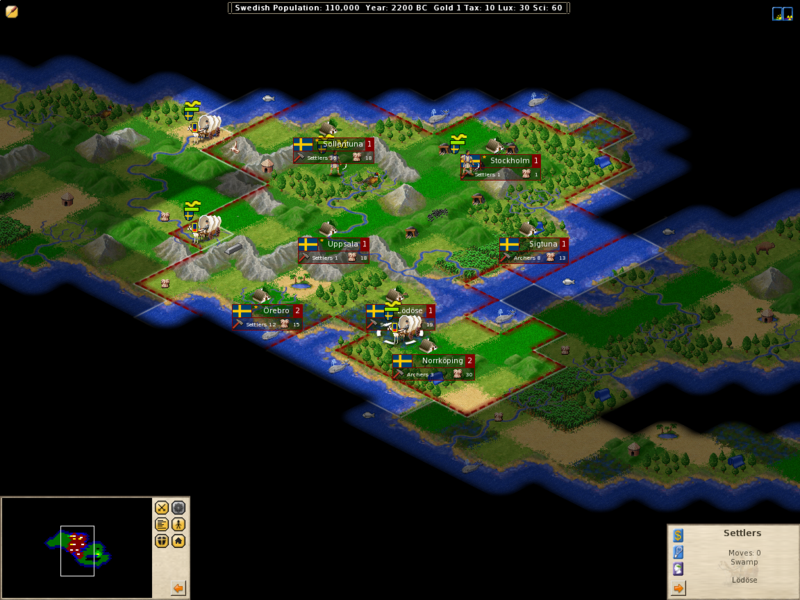
\includegraphics[height=2cm]{images/freeciv-logo.png}

\end{columns}
\end{frame} 

